\documentclass[11pt,a4paper]{article}
\usepackage[margin=24mm,headheight=14pt,includeheadfoot]{geometry}
\usepackage[T1]{fontenc}
\usepackage{amsmath,amsthm}
\usepackage{newtxtext,newtxmath,microtype}
\usepackage{booktabs,longtable,array,graphicx,pdflscape,caption,fancyhdr,xcolor,hyperref,placeins,float}
\definecolor{ink}{HTML}{23384D}
\hypersetup{colorlinks=true,linkcolor=ink,urlcolor=ink,citecolor=ink,
 pdftitle={Variance learning rates and backbones in KSIVI},pdfauthor={StatComp research investigation}}
\newtheorem{proposition}{Proposition}[section]
\newtheorem{corollary}[proposition]{Corollary}
\newcommand{\E}{\mathbb E}
\newcommand{\Var}{\operatorname{Var}}
\newcommand{\Cov}{\operatorname{Cov}}
\newcommand{\tr}{\operatorname{tr}}
\newcommand{\diag}{\operatorname{diag}}
\setlength{\parskip}{4pt}\setlength{\parindent}{1em}
\setlength{\tabcolsep}{4pt}\renewcommand{\arraystretch}{1.16}
\setlength{\emergencystretch}{1.5em}
\captionsetup{font=small,labelfont=bf,labelsep=period}
\pagestyle{fancy}\fancyhf{}
\fancyhead[L]{\small\itshape KSIVI: variance learning rates}
\fancyhead[R]{\small Atomic comparisons and mechanisms}
\fancyfoot[C]{\thepage}\renewcommand{\headrulewidth}{0.3pt}
\title{Can a Slower Variance Network Stabilize KSIVI?\\
\large Learning rates, shared features, and optimization budgets on the X-shaped target}
\author{StatComp research investigation}\date{12 October 2026}
\begin{document}\maketitle
\begin{abstract}
We test variance-specific Adam learning rates and variance architectures in the original StatComp KSIVI implementation on the X-shaped target. The campaign contains 190 primary runs at 50K updates and 36 checkpoint continuations to 200K. A shared variance-head LR of $10^{-5}$, with mean/backbone LR $10^{-3}$, reduces held-out sliced-Wasserstein error from $0.870\pm0.524$ to $0.129\pm0.044$, improving all five paired seeds. Its mean error is comparable to global variance (0.159); five seeds do not establish superiority. An independent linear variance map also performs well, while a large separate network is less reliable. Exact gradient-path identities, a finite-budget Adam reachability bound, and unchanged-marginal gradient-noise results for constant and Gaussian kernels explain why slower variance updates can help, why excessive slowing can fail, and why head LR does not control the entire shared variance function. Estimator, initialization, annealing, and continuation ablations delimit the result; there is no universal recommendation to decrease the variance LR.
\end{abstract}

\section{Question, findings, and the scope of the evidence}
The motivating suggestion is to reduce the variance learning rate while retaining
the mean learning rate. That suggestion has two distinct implementations:
slowing only a variance output layer on shared features, and slowing an entire
independent variance network. They need not have the same effect. We return to
the original StatComp model and training policy; the authors' alternative
defaults are not substituted for that policy in this campaign.

\begin{enumerate}
\item \textbf{The proposed slower head helps this conditional setting.} Reducing only the shared variance-head LR by $100\times$ improves all five held-out seeds and reduces their mean error by 85.2\%. The backbone retains both mean and variance gradient paths.
\item \textbf{The useful rate depends on the variance architecture.} Shared ratio 0.01 and separate ratio 0.03 were selected on discovery seeds. A separate linear variance model selects ratio 1; ratios 0.001--0.1 under-adapt in that model. Separation alone does not establish an advantage over global variance.
\item \textbf{Comparable marginal accuracy does not imply the same mechanism.} On held-out seeds the slow original estimator is competitive with global variance and Stein loss. A smaller head LR worsens the tested Stein treatment, so estimator changes and step-size changes are not interchangeable.
\item \textbf{Two distinct theoretical effects are necessary.} Smaller block steps reduce update noise at a fixed state, but must still permit the component variance to adapt from its initial value 1.3133. Shared features provide an additional full-rate route, and cumulative LR constrains what a slow independent network can reach.
\end{enumerate}

\begin{center}\small
\begin{tabular}{@{}>{\raggedright\arraybackslash}p{7cm}rr@{}}
\toprule
50K configuration & Discovery (3) & Held out (5) \\ \midrule
Shared, equal LR & $2.016\pm1.138$ & $0.870\pm0.524$ \\
Shared; LR ratio 0.01 & $0.178\pm0.086$ & $0.129\pm0.044$ \\
Separate 128x2; LR ratio 0.03 & $0.122\pm0.062$ & $0.240\pm0.159$ \\
Linear variance; LR ratio 1 & $0.101\pm0.032$ & $0.129\pm0.017$ \\
Global variance & $0.197\pm0.130$ & $0.159\pm0.079$ \\
Shared, Stein loss & $0.278\pm0.151$ & $0.262\pm0.178$ \\
Shared, floor 0.2 & $0.378\pm0.020$ & $0.397\pm0.012$ \\
Separate, equal LR & $0.915\pm0.516$ & $0.589\pm0.251$ \\
\bottomrule\end{tabular}
\end{center}

The statistical unit is an independently trained model. Monte Carlo samples
from one checkpoint do not count as additional training replications. Discovery
seeds select hyperparameters; held-out seeds assess those choices. Descriptive
means and sample standard deviations are reported, together with paired
per-seed outcomes. This is an exploratory investigation, not a preregistered
confirmatory significance test. No statement below establishes a universal
ordering of optimizers, architectures, or gradient estimators.

\section{The common model and loss}
Let $Z\sim N(0,I_2)$ and $U\sim N(0,I_2)$ be independent. StatComp samples
\[
 X=\mu_\phi(Z)+\sqrt{v_\phi(Z)}\odot U,\qquad
 v_\phi(Z)=\max\{10^{-4},\operatorname{softplus}(a_\phi(Z))\}.
\]
The mean uses two width-128 SiLU hidden layers. The global model replaces
$v_\phi(Z)$ by two learnable variance scalars. At initialization all matched
comparisons have the same mean function and constant variance
$\operatorname{softplus}(1)=1.3132616$, except explicitly labeled initialization
ablations. The effective mixing dimension is two: the production target binding
overrides the raw target-configuration entry.

Write $s_p=\nabla\log p$ and $s_c(X,Z)=\nabla_X\log q_\phi(X\mid Z)$.
The conditional Gaussian layer returns its negative score
$-s_c=U/\sqrt v$. With two independent batches of size $N=128$, the original
loss estimator is
\begin{equation}
 \widehat L_c=\frac1{N^2}\sum_{i,j} k_h(X_i,Y_j)
 \left(\alpha_t s_p(X_i)+\frac{U_i}{\sqrt{v(Z_i)}}\right)^T
 \left(\alpha_t s_p(Y_j)+\frac{U'_j}{\sqrt{v(Z'_j)}}\right).
 \label{eq:original}
\end{equation}
For a kernel fixed independently of these samples, the Fisher identity
$\E[s_c\mid X]=s_q(X)$ shows that its expectation is the squared KSD between
$q_\phi$ and $p_{\alpha_t}\propto p^{\alpha_t}$, under the usual integration
and differentiation conditions. This is the tractable conditional-score
formulation underlying KSIVI \cite{ksivi}. A larger conditional family need
not have a larger minimum population loss; our question concerns finite
stochastic optimization.

For the Gaussian kernel $k_h(x,y)=\exp[-\|x-y\|^2/(2h^2)]$, integration by
parts gives the conventional Stein form
\begin{equation}
 \widehat L_S=\frac1{N^2}\sum_{i,j} k_h(X_i,Y_j)
 \left[s_i^Ts'_j+\frac{(s_i-s'_j)^T(X_i-Y_j)}{h^2}
 +\frac2{h^2}-\frac{\|X_i-Y_j\|^2}{h^4}\right],
 \label{eq:stein}
\end{equation}
where $s_i=\alpha_t s_p(X_i)$. For independently fixed $h$, the two forms
have the same population objective, but different finite-batch gradients.
Neither form has a universally smaller gradient covariance.

Production training fits
$h^2=\operatorname{median}_{ij}\|X_i-Y_j\|^2/[2\log(N+1)]$ on each batch.
Original-loss runs differentiate this fitted width. Stein runs hold it fixed
during backpropagation, matching the earlier investigation. Thus the default
Stein comparison changes both estimator and bandwidth differentiation. We
include original-loss bandwidth-detachment controls and independently fixed
bandwidth probes; the fixed-kernel population identity is not asserted for a
sample-adaptive differentiated statistic.

\subsection{Relation to the original KSIVI guarantees}
The KSIVI analysis assumes controlled model derivatives and a uniform positive
lower bound on component standard deviations (Assumption 4.3), then establishes
gradient-variance bounds and an SGD stationarity guarantee under its full
assumptions (Theorems 4.7--4.8) \cite{ksivi}. Our small-variance limit leaves a
fixed uniformly nondegenerate parameter domain; it does not contradict those
results. The implemented $10^{-4}$ variance floor truncates that limit but can
still permit large noise constants. Stationarity also does not imply a small
transport error. Adam, annealing, and fitted bandwidths require further care
before applying a fixed-objective SGD theorem to these runs.

There is an additional exact boundary on this particular target: its log-density
does not have a globally bounded Hessian. In fact, with $c=1.8/0.76$,
\[
 \log p(x,y)=C-\frac{x^2+y^2}{0.76}+\log\cosh(cxy),\qquad
 \partial_{yy}\log p(R,0)=-\frac2{0.76}+c^2R^2.
\]
The last expression is unbounded as $R\to\infty$, so the target does not satisfy
the global Hessian condition in Assumption 4.2. Spatial autograd of the actual
target implementation checks the formula. This is a limitation on a direct
theorem application, not an explanation of the ordering of methods: all
methods in this campaign share the same target.

\section{What a variance learning rate can and cannot control}
\subsection{A head-only learning rate leaves another path active}
For a shared backbone $h_b(Z)$, write
\[
 \mu(Z)=M_\psi h_b(Z)+m_\psi,\qquad
 a(Z)=W_\omega h_b(Z)+c_\omega.
\]
The backbone gradient decomposes exactly as
\begin{equation}
 g_b=J_b\mu^T\partial_\mu\widehat L+J_b a^T\partial_a\widehat L
       =g_b^{\mu}+g_b^a.
 \label{eq:paths}
\end{equation}
A smaller learning rate for $(W,c)$ leaves the second term in the backbone's
gradient active at the backbone learning rate. Mean-driven backbone updates
also change the features read by the variance head.

\begin{proposition}[Exact functional drift decomposition]
For a fixed probe input, let $h'=h+\Delta h$, $W'=W+\Delta W$, and
$c'=c+\Delta c$ denote the values before and after one optimizer step. Then
\begin{equation}
 \Delta a=\underbrace{\Delta W h+\Delta c}_{\text{head}}
          +\underbrace{W\Delta h}_{\text{backbone}}
          +\underbrace{\Delta W\Delta h}_{\text{interaction}}.
 \label{eq:drift}
\end{equation}
Consequently, freezing a trained variance head does not generally freeze its
predicted variance on a changing shared backbone.
\end{proposition}
\begin{proof}
Expand $(W+\Delta W)(h+\Delta h)+(c+\Delta c)-(Wh+c)$.
When $\Delta W=\Delta c=0$, the remaining term is $W\Delta h$, which need
not vanish. At our constant initialization $W=0$, this route is initially
absent; after the head has learned, it can be present.
\end{proof}

At a fixed state, a first-order SGD calculation gives
$\Delta a\simeq-\eta_v J_\omega a\,g_\omega-\eta_bJ_b a\,g_b$.
As $\eta_v\to0$ with $\eta_b$ fixed, its conditional covariance tends to
$\eta_b^2J_b a\,\Cov(g_b)J_b a^T$ when this matrix is nonzero. Cross
covariances matter at finite $\eta_v$; the formula is not a universal positive
lower bound for every model or state. It does show why head LR alone cannot
guarantee control of functional variance noise.

For an independent variance network $a_\omega(Z)$, all of its parameters
receive $\eta_v$. To first order, both functional drift and stochastic
standard deviation scale with $\eta_v$ at a fixed state. This is genuine
control of the whole variance function, while also slowing its deterministic
learning. The gradient-path and trained-head-freeze probes test these routes
directly rather than inferring them from the final sample plots.

Our stop-gradient ablation detaches the shared features only along the
variance path. It removes $g_b^a$ but does not prevent $h_b$ from moving under
$g_b^\mu$. Moreover, this deliberately omits part of the shared model's
gradient: it is a routing heuristic, not an unbiased gradient of the original
shared objective. Separating backbones retains the full gradient of the new
parameterization.

\subsection{Different rates do not create gradient-estimation bias}
\begin{proposition}[Block learning rates and descent]
Let $L$ have a $\beta$-Lipschitz gradient, and let a stochastic gradient
$\widehat g$ at a fixed state have mean $g=\nabla L$ and covariance $\Sigma$.
For a deterministic positive block-diagonal learning-rate matrix $D$,
\[
 \E[D\widehat g]=Dg,
\]
and
\begin{equation}
 \E[L(\theta-D\widehat g)]\le L(\theta)-g^TDg
 +\frac\beta2\{g^TD^2g+\tr(D^2\Sigma)\}.
 \label{eq:descent}
\end{equation}
\end{proposition}
\begin{proof}
Apply the smoothness inequality to $-D\widehat g$, take expectations, and use
$\E[\widehat g\widehat g^T]=gg^T+\Sigma$.
\end{proof}

Thus changing a block LR preconditions the update; it does not by itself bias
the underlying gradient estimator. For that block, the expected first-order
movement scales as $\eta_v$, while the covariance of the SGD update scales as
$\eta_v^2$. Smaller steps can suppress noisy motion but also delay progress.
This is a local SGD statement. Adam's moment estimates are random and
history-dependent, so it is not claimed as an Adam convergence theorem.

For Adam, the learning rate multiplies the normalized direction
$\widehat m/(\sqrt{\widehat s}+\varepsilon)$ \cite{adam}. At fixed parameters,
historical moments, and a fresh stochastic gradient, scaling that block's LR
scales its parameter update. Multiplying its gradient by a constant is not
equivalent: the first and second moments approximately cancel the scale when
$\varepsilon$ is negligible. We therefore implement actual parameter groups,
not gradient multipliers. The legacy combined output layer is split into two
parameter blocks and concatenated for the same forward Linear operation.

\subsection{Separating backbones does not imply half the convergence speed}
Both networks receive gradients from the same loss and both are updated at
every iteration. There is no factor $1/2$ in either block's gradient. A simple
counterexample rules out a necessary twofold slowdown: for
$L(m,a)=(m^2+a^2)/2$, joint SGD and two simultaneously updated separate
blocks both obey $(m_{t+1},a_{t+1})=(1-\eta)(m_t,a_t)$ exactly. A separate
network can require more computation and can change conditioning and capacity;
those facts do not imply a fixed change in the number of optimizer steps.

\section{Why an arbitrarily slow variance network is not a complete solution}
\subsection{The initial scale must be able to shrink}
The X-shaped target is
\[
 p=\tfrac12N(0,\Sigma_+)+\tfrac12N(0,\Sigma_-),\qquad
 \Sigma_\pm=\begin{pmatrix}2&\pm1.8\\\pm1.8&2\end{pmatrix}.
\]
Its component eigenvalues are $3.8$ and $0.2$. If $S$ is an equiprobable sign,
$T\sim N(0,1)$, and $U\sim N(0,I_2)$ independently, then
\[
 X=\sqrt{1.8}\,T(1,S)^T+\sqrt{0.2}\,U
\]
has exactly this distribution. A global component variance of $0.2$ is
therefore sufficient with an unrestricted mixing distribution of means; a
finite continuous neural network approximates the discrete branch selection.

\begin{proposition}[An obstruction for frozen large component variance]
No mixing distribution of means convolved with $N(0,vI_2)$ can equal this
target when $v>0.2$.
\end{proposition}
\begin{proof}
In direction $w=(1,-1)^T/\sqrt2$, the target characteristic function is
$\varphi_p(tw)=\tfrac12e^{-0.1t^2}+\tfrac12e^{-1.9t^2}$. A representation
$X=M+\sqrt vU$ would require
$\varphi_M(tw)=\varphi_p(tw)e^{vt^2/2}$, which is unbounded as
$|t|\to\infty$ if $v>0.2$. Every characteristic function has modulus at most
one, a contradiction.
\end{proof}

More quantitatively, any such frozen-variance model satisfies
\[
 W_2(w^Tq,w^Tp)\ge W_1(w^Tq,w^Tp)
 \ge\sup_{t>0}\frac{[\varphi_p(tw)-e^{-vt^2/2}]_+}{t}.
\]
The last inequality follows from the Lipschitz constant $t$ of
$x\mapsto e^{itx}$ and $|\varphi_q(tw)|\le e^{-vt^2/2}$.
For the initial variance 1.31326, our numerical one-dimensional bound is
about 0.13535. It is a bound on this projection, not the averaged sliced
metric, and does not explain the full magnitude of an escaping training run.

This distinguishes a hard floor of $0.2$ from freezing the initial variance
near $1.3$. The floor permits shrinkage to the target's transverse scale;
freezing the initial value prevents that adaptation. Initialization at $0.2$
and its frozen control test this explanation directly.

\subsection{A finite-budget obstruction for a very slow linear variance head}
There is also a deterministic Adam bound that can make under-adaptation precise.
Consider Adam without weight decay, initialized with zero moments, with
$\beta_1^2<\beta_2$ and nonnegative numerical $\varepsilon$. For any coordinate,
\begin{equation}
 \left|\frac{\widehat m_t}{\sqrt{\widehat s_t}+\varepsilon}\right|
 \le C:=\frac{1-\beta_1}{\sqrt{(1-\beta_2)(1-\beta_1^2/\beta_2)}}.
 \label{eq:adam-bound}
\end{equation}
For our betas, $C=7.2703$. This bounds the coordinate update by $C\eta_t$
for every finite gradient sequence; no stochastic independence is assumed.

\begin{proposition}[Reachability bound for a linear variance model]
Let $a_j(Z)=w_j^TZ+b_j$, initially $w_j=0$ and $b_j=1$, with every variance
parameter assigned LR $r\eta_t$. Put $\delta=C r\sum_{t<T}\eta_t$.
On the latent region $B_M=\{\|Z\|_1\le M\}$, each variance is at least
$\ell=\operatorname{softplus}(1-(1+M)\delta)$. Since
$P(B_M)=\operatorname{erf}(M/2)^2=:P_M$, regardless of the trained mean,
\begin{equation}
 W_2(w^Tq_T,w^Tp)\ge
 \sup_{t>0}\frac{[\varphi_p(tw)-P_Me^{-\ell t^2/2}-(1-P_M)]_+}{t},
 \label{eq:reachable}
\end{equation}
where $w=(1,-1)^T/\sqrt2$. A positive right-hand side rules out an exact fit
within the specified optimization budget.
\end{proposition}
\begin{proof}
For completeness, Cauchy--Schwarz applied to the two weighted gradient moments
gives the squared bound
\[
 C_t^2=\frac{(1-\beta_1)^2}{(1-\beta_1^t)^2}
 \frac{1-\beta_2^t}{1-\beta_2}
 \frac{1-(\beta_1^2/\beta_2)^t}{1-\beta_1^2/\beta_2}.
\]
The inequality $(1-x)(1-y)\le(1-\sqrt{xy})^2$, with
$x=\beta_2^t$ and $y=(\beta_1^2/\beta_2)^t$, shows $C_t\le C$.
Summing coordinate updates gives $|w_{jk}|\le\delta$ and $|b_j-1|\le\delta$,
so $a_j(Z)\ge1-(1+M)\delta$ on $B_M$. Orthogonal rotation of a standard
bivariate Gaussian gives $P(B_M)=\operatorname{erf}(M/2)^2$.
Conditional noise in direction $w$ has variance $(v_1+v_2)/2\ge\ell$ on
$B_M$. Therefore
$|\varphi_{q_T}(tw)|\le P_Me^{-\ell t^2/2}+(1-P_M)$, independently of
the conditional means. The Lipschitz characteristic-function argument from
the previous subsection gives \eqref{eq:reachable}.
\end{proof}

For $r=0.001$, $T=50K$, and $M=3$, the coordinate displacement is at most
about $0.0723$ and $P_M\simeq0.9334$. The resulting projection bound is
strictly positive. Retaining the original decay through 200K scarcely changes
it. The recorded numerical checks give the full bounds for the restart policy
and additional rates. These are bounds for the linear variance architecture,
in exact arithmetic; they are not bounds for an unrestricted changing shared
feature map. Linear-head runs at ratios 0.001 and 0.003 are included to test
this predicted finite-budget limitation. The result shows why a universally
beneficial prescription to decrease the variance LR cannot hold, even before
considering stochastic gradient variance.

\subsection{Representation noise can grow without a worse marginal}
The conditional score has the exact coordinate second moment
$\E[s_{c,j}^2]=\E[1/v_j(Z)]$. This is a diagnostic of representation noise,
not a bound on every parameter-gradient variance or a proof of poor marginal
fit. The following solvable example makes that distinction explicit.

\begin{proposition}[An exact finite-batch gradient-noise example]
Let $p=N(0,1)$ and, for $0<v<1$, represent $q_v=p$ as
$X=\sqrt{1-v}\,E+\sqrt v\,U$, where $E,U$ are independent standard Normals.
Take the constant kernel $k=1$, two independent batches of size $N$, and
differentiate with respect to $r=\log v$ while preserving this representation.
Both population objectives are zero for every $v$, but their stochastic
gradient variances are
\begin{align}
 \Var(\widehat g_c)&=\frac{2+v-v^2}{2N^2v^2},\\
 \Var(\widehat g_S)&=\frac{v}{2(1-v)N^2}.
 \label{eq:proxy}
\end{align}
\end{proposition}
\begin{proof}
Put $F=-X+U/\sqrt v$ and $B=\partial_rF$. Direct differentiation gives
\[
 F=-\sqrt{1-v}E+\frac{1-v}{\sqrt v}U,\quad
 B=\frac{v}{2\sqrt{1-v}}E-\frac{1+v}{2\sqrt v}U.
\]
Hence $A=\Var(F)=(1-v)/v$,
$C=\Var(B)=(1+v-v^2)/[4v(1-v)]$, and
$D=\Cov(F,B)=-1/(2v)$. The original gradient is
$\bar B\bar F'+\bar F\bar B'$, with independent primed batches, so its
variance is $2(AC+D^2)/N^2$, giving the first expression.
For the Stein form, $k=1$ removes all spatial kernel derivatives and the loss
is $\bar X\bar X'$. Here $\Var(X)=1$,
$\Var(\partial_rX)=v/[4(1-v)]$, and
$\Cov(X,\partial_rX)=0$. The same calculation gives the second expression.
\end{proof}

The constant kernel is an analytically solvable proxy, not the characteristic
Gaussian kernel used in training. Independent fixed-bandwidth RBF simulations
with the same unchanged marginal check whether the mechanism also appears
with the training kernel family. The formulas prove a possible noise mechanism,
not a universal RBF variance ordering: near $v=0.8$ even the constant-kernel
ordering reverses. A small learning rate changes update noise, while Stein
integration removes the explicit component-score terms themselves.

\begin{proposition}[Small-variance asymptotics for the Gaussian kernel]
Let $p=q_v=N(0,I_d)$ be represented as
$X_v=\sqrt{1-v}\,E+\sqrt v\,U$ with independent standard Gaussian vectors,
and use two independent batches of fixed size $N$. For fixed $h>0$ and
$r=\log v$, the original Gaussian-kernel gradient satisfies
\begin{equation}
 \lim_{v\downarrow0}v^2\Var(\partial_r\widehat L_c)
 =\frac{d}{N^2}\left(1+\frac4{h^2}\right)^{-d/2}>0,
 \qquad \Var(\partial_r\widehat L_S)=O(v).
 \label{eq:rbf-asymptotic}
\end{equation}
Both population gradients are zero for every $v$. Thus the noise divergence
also occurs with a characteristic Gaussian kernel, without changing the
marginal distribution or the population objective.
\end{proposition}
\begin{proof}
For the original estimator $F_v=-X_v+U/\sqrt v$,
$F_v=U/\sqrt v+O_{L^p}(1)$ and
$\partial_r F_v=-U/(2\sqrt v)+O_{L^p}(\sqrt v)$ for every finite $p$.
Also $\partial_rX_v=O_{L^p}(\sqrt v)$. Gaussian kernel derivatives are
bounded, so differentiation of its factor contributes only
$O_{L^2}(v^{-1/2})$ to the gradient. Therefore
\[
 v\partial_r\widehat L_c\ \longrightarrow\
 -\frac1{N^2}\sum_{i,j}k_h(E_i,E'_j)U_i^TU'_j
 \quad\text{in }L^2.
\]
All cross terms except identical $(i,j)$ vanish after conditioning on the
latent $E$'s and taking expectations over independent centered $U$'s.
The limiting variance is
$d\E[k_h(E,E')^2]/N^2$.
Since $E-E'\sim N(0,2I_d)$, this kernel moment equals
$(1+4/h^2)^{-d/2}$. The Stein integrand and its first spatial derivatives
have uniformly bounded Gaussian moments, and its only $r$ dependence is
through $X_v,Y_v$. Its gradient is consequently $O_{L^2}(\sqrt v)$,
which gives the stated variance order. The $L^2$ limit also justifies passage
of the mean and variance; the common population loss is identically zero.
\end{proof}

For $d=2$, $N=128$, and $h=0.75$, the leading coefficient is approximately
$1.5050\times10^{-5}$. Numerical simulations compare $v^2$ times the original
gradient variance with this coefficient, rather than relying only on a visual
log--log slope. This theorem concerns a specified marginal-preserving direction;
it is not a lower bound for every parameter direction in a trained neural model.

\section{Experimental protocol and atomic controls}
All primary results use 50,000 updates. The fixed policy is Adam
$(0.9,0.999)$, mean LR $10^{-3}$, two batches of 128, StepLR multiplier 0.9
per 1,000 updates, and score annealing
$\alpha_t=0.1+0.9\min(t/25000,1)$. The Gaussian distance arithmetic remains
the StatComp implementation. Diagnostic RNG is isolated. We omit a
diagnostic-only bandwidth-to-CPU synchronization in the fast update; equality
of the loss, gradients, and production optimizer update is checked on CPU and
GPU. No gradient clipping, EMA, or log-density regularization is introduced.

Discovery sweeps variance/mean LR ratios
$\{0,0.001,0.003,0.01,0.03,0.1,0.3,1,3\}$ with seeds 42--44, for shared
and separate width-128 two-layer backbones. For the shared model, only the
variance output parameters receive this rate; for a separate model, the
entire variance network receives it. Both networks are updated every step.
Separate width-32, one-hidden-layer, linear, and shared stop-gradient
alternatives are each tested at ratios $\{0.01,0.1,1\}$. Initial mean
functions, constant variances, and training-noise seeds are paired.

The minimum mean discovery SW$_2$ at a positive LR selects one shared, one
separate, and one alternative configuration. That selection is recorded
before held-out seeds 45--49. Held-out controls include equal-LR shared and
separate models, global variance, Stein loss, and a $0.2$ floor. Further
paired ablations change only annealing, initial variance, bandwidth detachment,
or estimator/floor for the selected head LR. Every such change is labeled.

Training diagnostics use 10,000 samples and 128 projection directions.
Independent final evaluation uses 20,000 samples and 128 directions, plus a
second 10,000-sample check. Forward KL uses 2,048 exact target points and
an empirical Gaussian mixture for $q$: mixture sizes 8,192, 16,384, and
65,536 are checked, and 262,144 is used when the last change exceeds 0.02.
The last change is retained; the pointwise Monte Carlo standard error does
not include all mixture-approximation uncertainty. Held-out KSD uses 16
independent cross-batch estimates, 256 samples per batch, at independently
fixed bandwidths $0.5,0.75,1.5$. Negative finite-sample estimates are retained.

\subsection{Why update counts and learning-rate budgets are both reported}
With $\eta_t=10^{-3}0.9^{\lfloor t/1000\rfloor}$, the first 50,000 updates
have total nominal LR
\[
 S_{50K}=1000\cdot10^{-3}\frac{1-0.9^{50}}{1-0.9}=9.94846.
\]
The sum through 200,000 is almost 10, adding only 0.518\% to $S_{50K}$.
These sums are not actual Adam path lengths, but they show why extra decayed
updates need not compensate for a smaller variance LR. We fork exact 50K
checkpoints, including Adam and RNG state, to two labeled continuations:
retained StepLR decay, or a restart at mean LR $10^{-4}$ with the original
variance/mean LR ratio, held constant. The latter adds nominal mean LR 15
over the next 150K updates. Its improvement cannot be attributed to update
count alone. All continuations are compared at 100K and 200K, and no run
exceeds 200K updates.

\section{Results and ablations}
\subsection{Learning-rate sweep: improvement has a finite useful range}
On discovery seeds, the shared equal-LR mean error is 2.016, versus 0.178 at ratio 0.01. Shared ratios 0.003, 0.01, and 0.03 yield means 0.204, 0.178, and 0.185. This is a useful region rather than evidence that 0.01 is an exact optimum. Ratio 0.001 is more variable, and ratio zero fails. The independent width-128 two-layer variance network instead has mean errors 8.980, 4.239, and 0.122 at ratios 0.001, 0.003, and 0.03. High ratios can also fail; the separate ratio-3 mean is 4.562. Thus neither a monotone LR rule nor separation alone describes the observations.

\begin{figure}[H]\centering
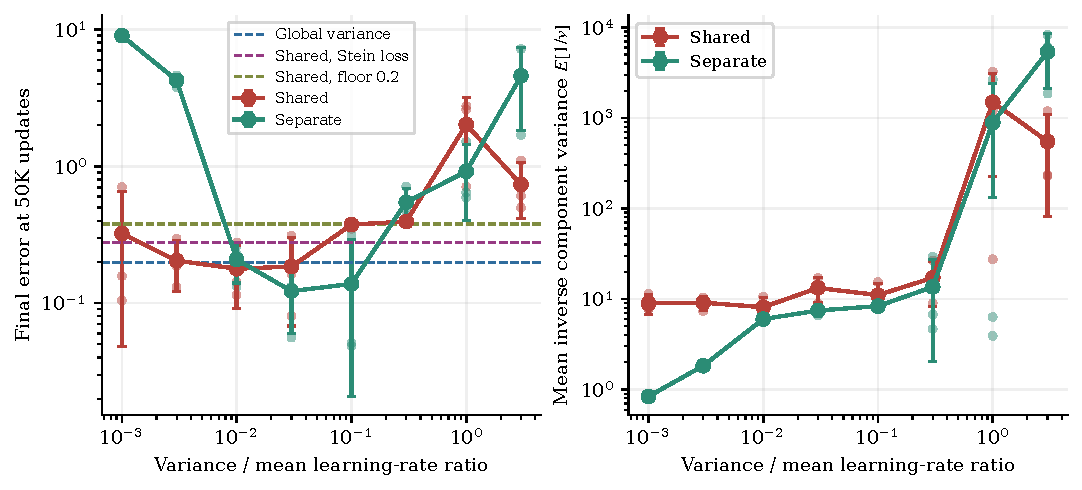
\includegraphics[width=\linewidth]{figures/learning_rate_sweep.pdf}
\caption{Three paired discovery seeds at 50K updates. Lines are arithmetic means; dots are runs. Error bars are sample SD, with lower ends clipped for logarithmic display only. The right panel measures component-score second moments through $\E[1/v]$, not marginal error. Zero-LR controls are tabulated in the appendix.}\label{fig:learning_rate_sweep}
\end{figure}
\FloatBarrier\subsection{Prospective held-out comparison}
Selection was committed at \texttt{808b97f} before seeds 45--49 were launched. The shared slow head improves all five paired equal-LR controls. It beats global variance on 3/5 seeds and Stein loss on 3/5. The separate selected network improves its own equal-LR control on 4/5 seeds, but has held-out mean 0.240, compared with 0.129 for the slow shared head. The selected linear variance map has mean 0.129, with all five errors between 0.101 and 0.145. These observations favor a slow shared output layer or restricted variance capacity as practical candidates. They do not show either candidate is statistically superior to global variance.

\begin{figure}[H]\centering
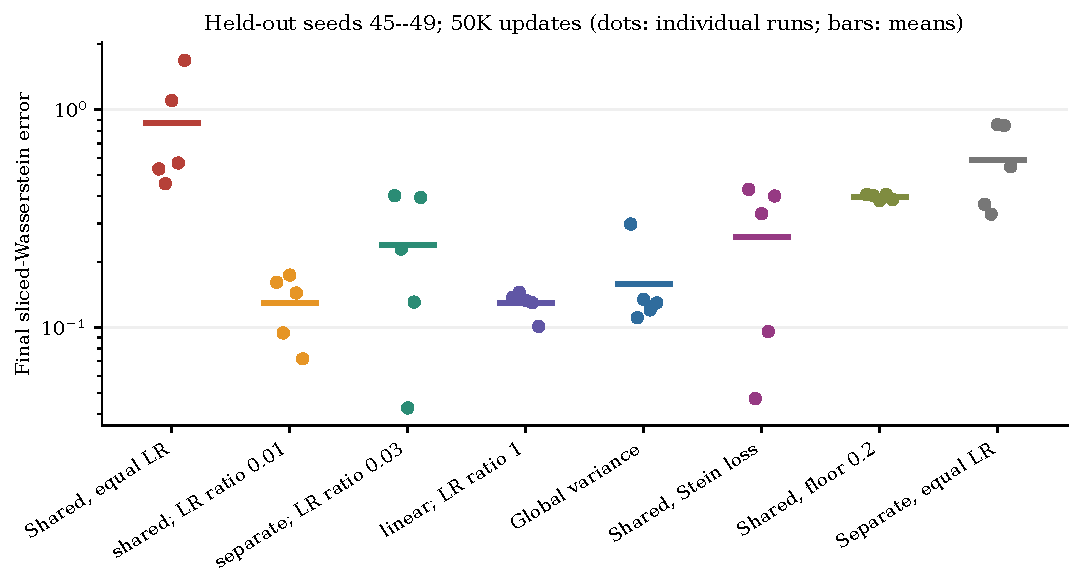
\includegraphics[width=\linewidth]{figures/heldout_comparison.pdf}
\caption{Five held-out training seeds, all at 50K optimizer updates. Each dot is one trained model. Horizontal bars are means. Hyperparameter selection uses none of these seeds.}\label{fig:heldout_comparison}
\end{figure}
\begin{table}[H]\centering\small
\caption{Paired held-out differences in training-diagnostic SW$_2$; negative favors the slow shared head.}
\begin{tabular}{@{}>{\raggedright\arraybackslash}p{7cm}rrr@{}}
\toprule
Slow shared minus comparator & Mean difference & SD of differences & Wins \\ \midrule
Shared, equal LR & -0.741 & 0.543 & 5/5 \\
Separate 128x2; LR ratio 0.03 & -0.111 & 0.185 & 3/5 \\
Linear variance; LR ratio 1 & -0.000 & 0.038 & 2/5 \\
Global variance & -0.030 & 0.071 & 3/5 \\
Shared, Stein loss & -0.132 & 0.175 & 3/5 \\
Shared, floor 0.2 & -0.268 & 0.044 & 5/5 \\
Separate, equal LR & -0.460 & 0.235 & 5/5 \\
\bottomrule\end{tabular}\end{table}
\FloatBarrier\subsection{Changing the variance backbone or its gradient route}
The selected alternative is an independent affine map $a(Z)=WZ+c$ with only six variance parameters, versus two for global variance. It is a genuine conditional family, but the learned conditional variation is measured separately below. Its good result therefore need not imply that a rich conditional variance network was necessary. At ratio 0.01 the stop-gradient shared variant has mean error 6.682, compared with 0.178 with the full shared gradient. At ratio 0.1 it recovers to 0.365. Removing the variance-to-backbone gradient is therefore not a harmless way to implement a slower variance function: here it removes useful adaptation under the finite budget. The comparison is a causal routing intervention with identical forward architecture, but it also changes the update rule as described in Section 3.

\begin{figure}[H]\centering
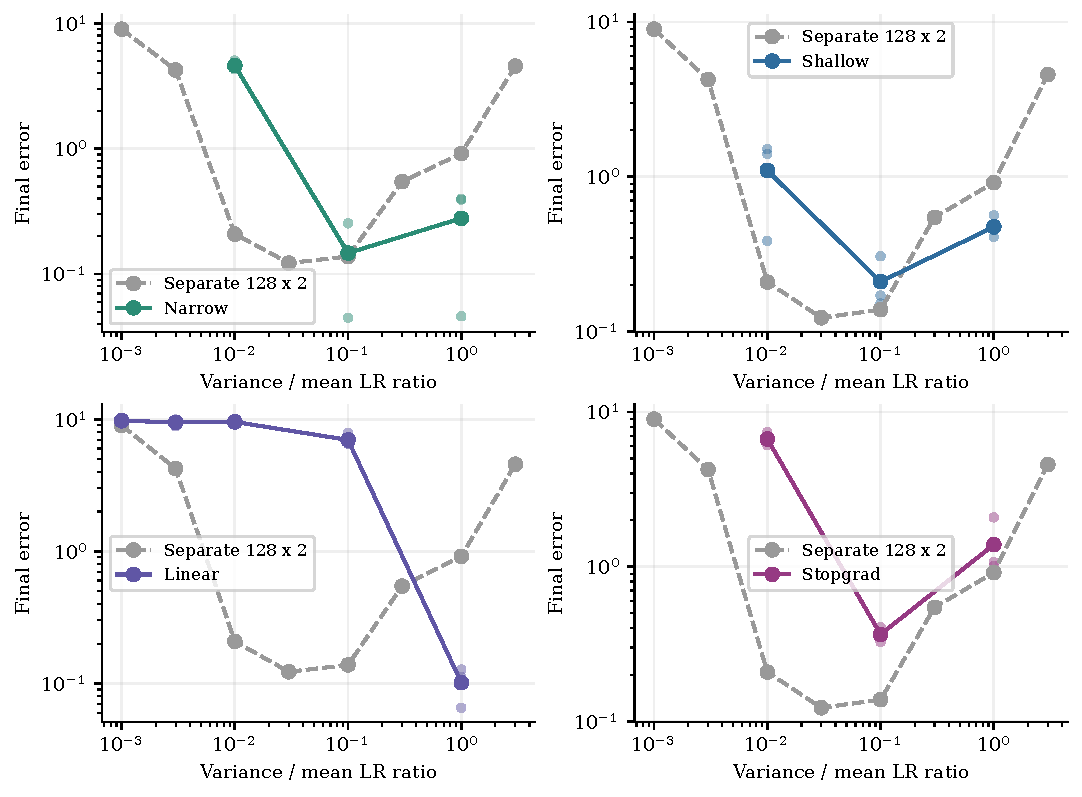
\includegraphics[width=\linewidth]{figures/architecture_ablation.pdf}
\caption{Variance architecture ablations, discovery seeds at 50K. The mean network remains width 128 with two hidden layers. Width 32, one hidden layer, and no hidden layer change only the variance branch relative to the separate network; stop-gradient changes only routing relative to shared features. Gray curves show the separate width-128 two-layer reference.}\label{fig:architecture_ablation}
\end{figure}
\begin{table}[H]\centering\small
\caption{Parameter counts. The common mean-only network has 17,154 parameters. For shared features, the last column counts additional variance output parameters; the backbone still receives both paths.}
\begin{tabular}{@{}>{\raggedright\arraybackslash}p{8cm}rr@{}}
\toprule
Variance architecture & Total parameters & Variance parameters \\ \midrule
Global variance & 17156 & 2 \\
Shared, equal LR & 17412 & 258 \\
Separate, equal LR & 34308 & 17154 \\
Separate 32x2; LR ratio 1 & 18372 & 1218 \\
Separate 128x1; LR ratio 1 & 17796 & 642 \\
Linear variance; LR ratio 1 & 17160 & 6 \\
\bottomrule\end{tabular}\end{table}
\FloatBarrier\subsection{Atomic initialization, annealing, kernel, and estimator controls}
\textbf{Initialization and freezing.} Frozen variance 1.3133 gives mean error 9.467; frozen variance 0.2 gives 0.264. Initializing the selected separate network at 0.2 changes its mean from 0.122 to 0.064. This supports the need to adapt the initially broad component noise. The effect is not uniform: initialization at 0.2 does not improve every selected shared or global run. A floor and a frozen initial scale are different interventions.

\textbf{Annealing.} Removing score annealing changes the shared equal-LR mean from 2.016 to 0.622, but changes global variance from 0.197 to 0.535, the selected separate network from 0.122 to 0.264, and Stein from 0.278 to 0.533. Annealing interacts with the optimizer state and model; disabling it is not a general cure.

\textbf{Estimator and bandwidth.} The slow-head original-loss mean is 0.178. Its bandwidth-detached control has mean 0.241, while Stein with that same slow head has mean 0.480. The latter two share the bandwidth-detachment policy, providing the cleaner estimator contrast. The tested slow head does not improve Stein. Adding a 0.2 floor to the slow original head gives mean 0.142, versus 0.378 for a floor at equal LR. This combination was evaluated only on discovery seeds; it is not a held-out recommendation.

\begin{figure}[H]\centering
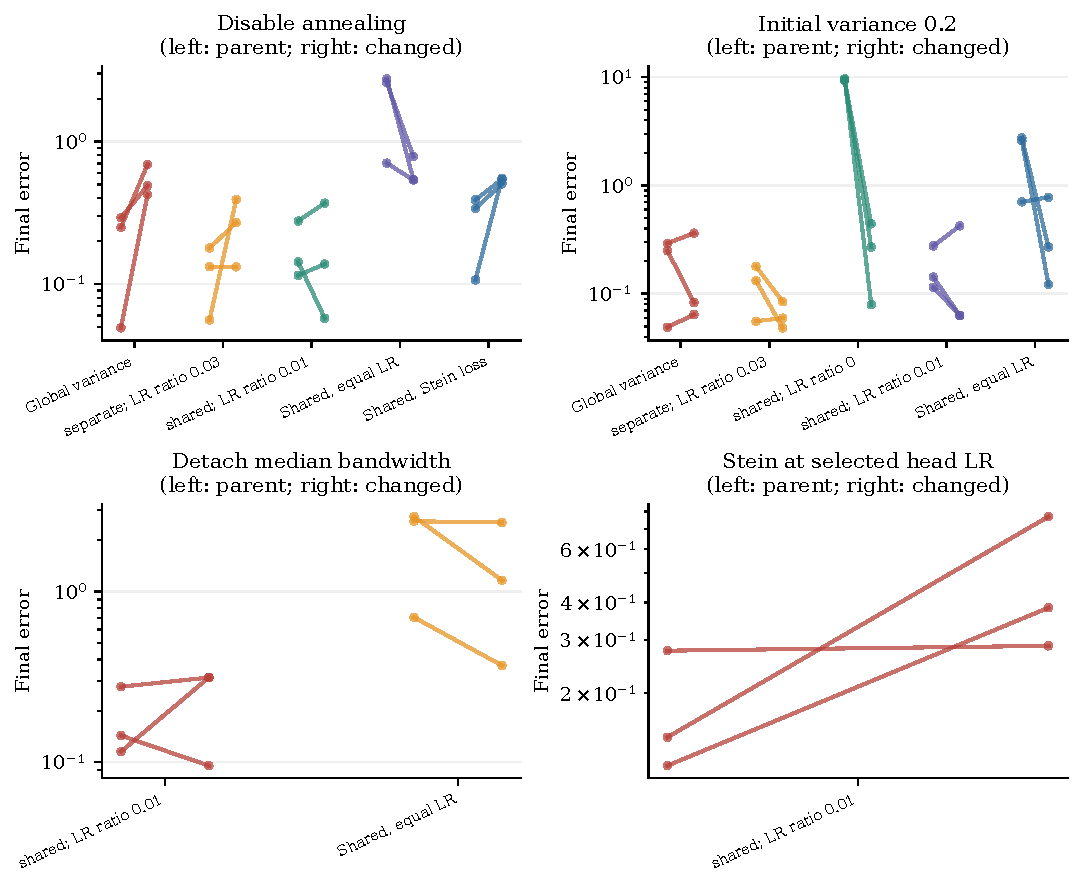
\includegraphics[width=\linewidth]{figures/atomic_ablations.pdf}
\caption{Paired atomic changes at 50K updates. Each short segment connects the same seed in the parent (left) and changed (right) configuration. A decrease is an improvement. The appendix includes all 14 contrasts, including the floor and frozen-variance controls.}\label{fig:atomic_ablations}
\end{figure}
\FloatBarrier\subsection{50K, 100K, and 200K: continued decay versus restart}
All continuations start from the exact 50K model, Adam moments, and training RNG state. Each branch adds 150K updates. The table and Figure~\ref{fig:extended_budgets} compare retained decay with a constant $10^{-4}$ mean LR restart; variance LR ratios remain fixed. Continuation evidence uses discovery seeds and should not be read as a new held-out ranking.

\begin{table}[H]\centering\small
\caption{Update-matched continuation results; means $\pm$ sample SD over three seeds. Restart changes cumulative LR as well as running longer.}
\begin{tabular}{@{}>{\raggedright\arraybackslash}p{4.2cm}rrrr@{}}
\toprule
Parent & Policy & 50K & 100K & 200K \\ \midrule
Global variance & decay & $0.197\pm0.130$ & $0.192\pm0.127$ & $0.192\pm0.127$ \\
Global variance & restart1e-4 & $0.197\pm0.130$ & $0.115\pm0.025$ & $0.103\pm0.036$ \\
Linear variance; LR ratio 0.001 & decay & $9.747\pm0.139$ & $9.803\pm0.135$ & $9.803\pm0.135$ \\
Linear variance; LR ratio 0.001 & restart1e-4 & $9.747\pm0.139$ & $11.410\pm0.567$ & $17.826\pm3.346$ \\
Separate 128x2; LR ratio 0.03 & decay & $0.122\pm0.062$ & $0.121\pm0.059$ & $0.121\pm0.059$ \\
Separate 128x2; LR ratio 0.03 & restart1e-4 & $0.122\pm0.062$ & $0.104\pm0.044$ & $0.109\pm0.048$ \\
Shared; LR ratio 0.01 & decay & $0.178\pm0.086$ & $0.176\pm0.086$ & $0.176\pm0.086$ \\
Shared; LR ratio 0.01 & restart1e-4 & $0.178\pm0.086$ & $0.106\pm0.003$ & $0.109\pm0.015$ \\
Shared, equal LR & decay & $2.016\pm1.138$ & $1.985\pm1.118$ & $1.985\pm1.118$ \\
Shared, equal LR & restart1e-4 & $2.016\pm1.138$ & $1.680\pm0.755$ & $1.461\pm0.745$ \\
Shared, Stein loss & decay & $0.278\pm0.151$ & $0.276\pm0.154$ & $0.276\pm0.154$ \\
Shared, Stein loss & restart1e-4 & $0.278\pm0.151$ & $0.253\pm0.176$ & $0.225\pm0.148$ \\
\bottomrule\end{tabular}\end{table}
\begin{figure}[H]\centering
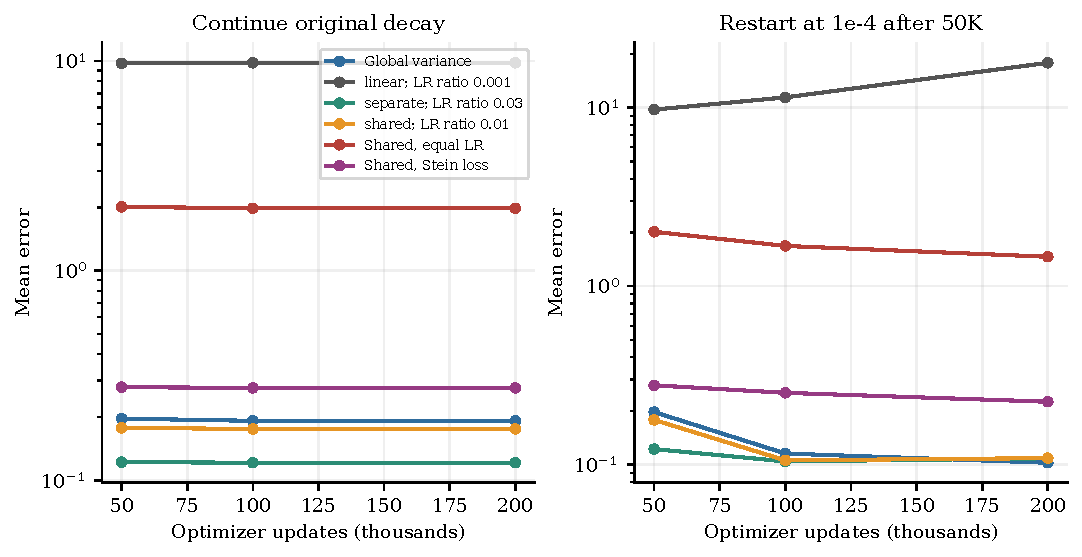
\includegraphics[width=\linewidth]{figures/extended_budgets.pdf}
\caption{Matched checkpoint continuations. The original decay has almost exhausted its nominal LR budget at 50K. Restart supplies a materially different budget, while keeping the estimator and variance LR ratio unchanged. The linear ratio-0.001 control tests the finite-budget obstruction.}\label{fig:extended_budgets}
\end{figure}
At 200K with restart, mean errors are 0.109 for the selected shared head, 0.109 for the selected separate network, 0.103 for global variance, and 0.225 for Stein. The shared equal-LR parent remains much worse at 1.461. The very slow linear ratio-0.001 model changes from 9.747 at 50K to 17.826; more optimization does not repair its frozen-scale-like constraint. The reachability theorem rules out an exact fit in this control but does not predict the large magnitude of its observed escape.



\section{Mechanistic evidence and boundaries}
\FloatBarrier\subsection{Marginal fit and inverse-variance moments are distinct}
The shared equal-LR discovery mean $\E[1/v]$ is 1490.1, compared with 8.12 for the slow head. Stein training nevertheless reaches 1488.0, with much better marginal error than the equal-LR original estimator. Conversely, the frozen wide-variance model has small inverse variance and poor fit. These controls reject an explanation based solely on the size of component variance: the score representation, update dynamics, and necessary variance adaptation all matter.

\begin{figure}[H]\centering
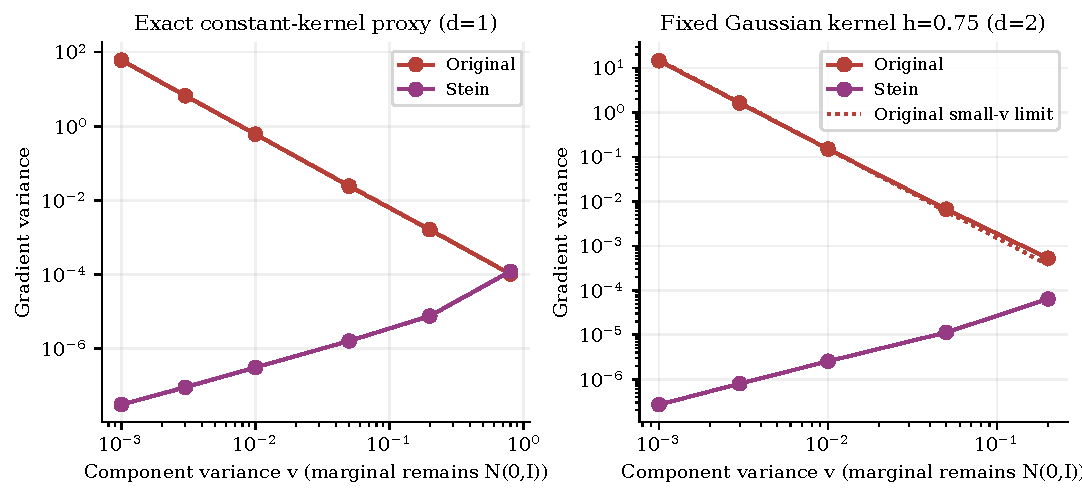
\includegraphics[width=\linewidth]{figures/representation_noise.pdf}
\caption{Unchanged-marginal controls: all representations have the same standard Gaussian marginal. Left: 20,000 replicated gradients and the exact constant-kernel formulas (dashed), two batches of 128. Right: 512 replications with fixed Gaussian bandwidth 0.75. The derivative follows $\log v$ while preserving the marginal; these are mechanism controls, not additional trained X-shaped models.}\label{fig:representation_noise}
\end{figure}
Increasing batch size can reduce this noise, but cannot give a variance-uniform guarantee at a fixed batch size. In the exact proxy, original variance behaves as $(Nv)^{-2}$ when $v$ is small; keeping it bounded requires $N$ to grow at least on the order of $1/v$. The Stein proxy instead has variance of order $v/N^2$ in that limit. This is an exact counterexample to a uniform fixed-batch cure, not a claim that every neural-network gradient has the same batch-size law. No new batch-size sweep is used to infer an X-shaped threshold.

The Gaussian-kernel theorem predicts $v^2\Var(\widehat g_c)\to1.50498e-05$. The observed ratios to that limit are 0.9744 at $v=0.003$, 0.9659 at $v=0.001$. Thus the fixed-RBF simulation checks a proved coefficient, with the same Gaussian marginal throughout. A slower LR acts on the resulting update; it does not remove this estimator-level divergence.

\subsection{Independent marginal metrics and density-approximation checks}
\begin{table}[H]\centering\small
\caption{Independent evaluation of the same five held-out trained models. SD is across training seeds; KSD values are means of unbiased cross-batch estimates.}
\begin{tabular}{@{}>{\raggedright\arraybackslash}p{6.1cm}rrr@{}}
\toprule
Held-out configuration & SW$_2$ (20K) & Forward KL & KSD$^2$, $h=.75$ \\ \midrule
Shared, equal LR & $0.859\pm0.496$ & $0.895\pm0.260$ & 0.0162 \\
Shared; LR ratio 0.01 & $0.127\pm0.039$ & $0.056\pm0.049$ & -0.000461 \\
Separate 128x2; LR ratio 0.03 & $0.236\pm0.163$ & $0.350\pm0.388$ & 0.000541 \\
Linear variance; LR ratio 1 & $0.127\pm0.013$ & $0.061\pm0.023$ & 0.000554 \\
Global variance & $0.159\pm0.079$ & $0.121\pm0.144$ & -5.09e-05 \\
Shared, Stein loss & $0.263\pm0.175$ & $0.296\pm0.278$ & 0.00314 \\
Shared, floor 0.2 & $0.395\pm0.011$ & $0.531\pm0.033$ & 0.0049 \\
Separate, equal LR & $0.576\pm0.219$ & $0.661\pm0.486$ & 0.0102 \\
\bottomrule\end{tabular}\end{table}
The independent samples preserve the main comparisons without recycling the selection metric sample. Across all 262 evaluated checkpoints, 15 retain a last KL mixture-refinement change above 0.02; the maximum is 1.36. Those density estimates are flagged in the CSV and must not be treated as exact KL. None of the held-out 50K comparisons has a final refinement change above 0.02. Independent fixed-bandwidth KSD values and their Monte Carlo standard errors are retained at all three widths, including negative estimates. KSD, forward KL, and SW$_2$ measure different aspects of fit and need not order all bad runs identically. For example, if $q_R=(1-\epsilon)p+\epsilon r_R$, then $D_{KL}(p\Vert q_R)\le-\log(1-\epsilon)$ even when $r_R$ moves arbitrarily far away. Transport error can then grow without bound. This elementary example explains why a modest forward KL alone cannot rule out escaped mass; it does not assert that a particular checkpoint has this exact mixture form.

The linear variance model has held-out mean conditional coefficient of variation 0.0332 (averaged over dimensions and seeds; range 0.0143--0.0608). These small coefficients mean the learned variance is close to global on typical latent inputs. A good score for this low-capacity map is therefore not evidence that rich conditional variance was needed.

\subsection{Gradient paths and functional drift at trained checkpoints}
\begin{table}[H]\centering\small
\caption{Discovery checkpoints at 50K. Norms/cosines use the original loss and average 32 stochastic gradients per model and then training seeds. Freeze drift uses a standardized local mean LR 0.001, with the variance block frozen; it is an intervention, not an additional training run.}
\begin{tabular}{@{}>{\raggedright\arraybackslash}p{4.4cm}rrrr@{}}
\toprule
Checkpoint & Mean path norm & Variance path norm & Mean cosine & Freeze drift RMS \\ \midrule
Shared, equal LR & 14.4 & 5.99 & 0.013 & 0.0199 \\
Shared; LR ratio 0.01 & 0.136 & 0.0206 & -0.002 & 0.00232 \\
Separate 128x2; LR ratio 0.03 & 0.103 & 0 & 0.000 & 0 \\
Shared stop-gradient; LR ratio 0.01 & 0.116 & 0 & 0.000 & 0.0023 \\
Linear variance; LR ratio 1 & 0.0797 & 0 & 0.000 & 0 \\
\bottomrule\end{tabular}\end{table}
The measured gradient decomposition has maximum reported mean relative residual 4.48e-07; the raw-output drift identity has maximum absolute residual 5.75e-14. A trained shared variance head can keep changing its output when its own LR is zero. The independent variance network has exactly zero drift when its entire block is frozen. Stop-gradient can still drift through mean-driven features. These interventions directly establish the remaining route. Gradient-path cosine alone would not prove it, and its sign is not a universal explanation of the training outcome.

\begin{table}[H]\centering\small
\caption{Unfrozen standardized local step and stochastic backbone gradients at the same checkpoints. Feature drift denotes the $W\Delta h$ term, including independent variance features for the separate network. Noise traces concern the original loss and only the mean backbone; a zero variance-path trace in separate/routed models is structural, not zero noise in their variance branch.}
\begin{tabular}{@{}>{\raggedright\arraybackslash}p{4.2cm}rrrr@{}}
\toprule
Checkpoint & \shortstack{Head drift\\RMS} & \shortstack{Feature drift\\RMS} & \shortstack{Mean-path\\noise trace} & \shortstack{Var-path\\noise trace} \\ \midrule
Shared, equal LR & 0.021 & 0.0199 & 467 & 75.8 \\
Shared; LR ratio 0.01 & 0.000381 & 0.00232 & 0.0195 & 0.000544 \\
Separate 128x2; LR ratio 0.03 & 0.000544 & 0.000613 & 0.0119 & 0 \\
Shared stop-gradient; LR ratio 0.01 & 0.000249 & 0.0023 & 0.0158 & 0 \\
Linear variance; LR ratio 1 & 0.000318 & 0 & 0.00722 & 0 \\
\bottomrule\end{tabular}\end{table}
The slow shared head has feature-driven raw-variance drift larger than head-driven drift in this local intervention, confirming that its variance function is not simply frozen. Equal-LR shared checkpoints have much larger measured backbone noise traces than the selected slow-head checkpoints. These are comparisons between different learned states: they support the noise mechanism but do not isolate a same-state causal effect of the LR.

\begin{figure}[H]\centering
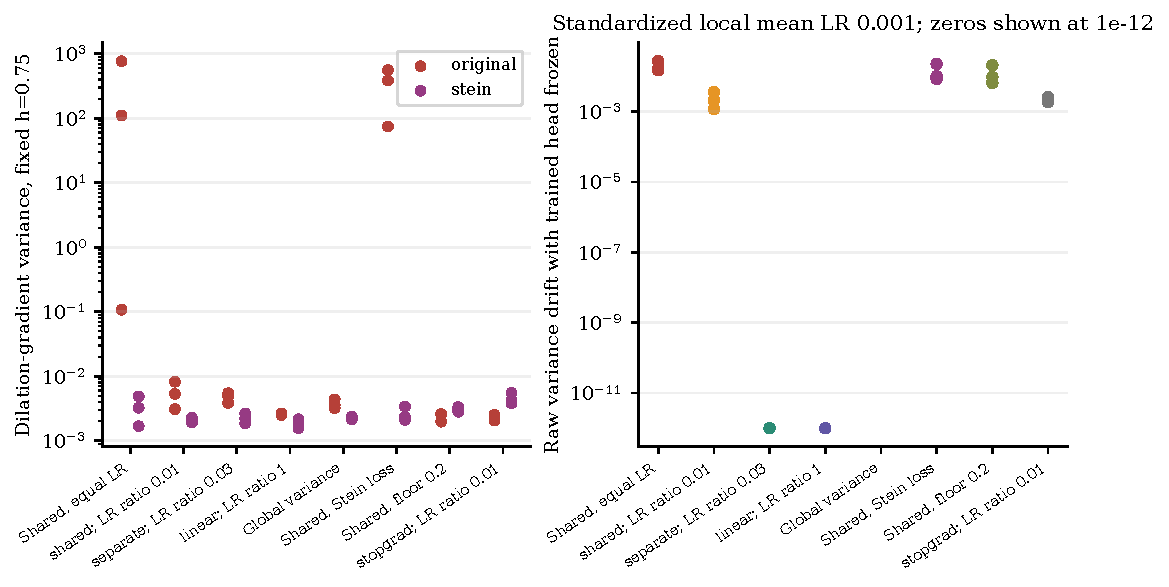
\includegraphics[width=\linewidth]{figures/trained_mechanisms.pdf}
\caption{Trained-checkpoint probes on discovery seeds. Left: gradient variance for a common marginal-dilation direction, using independently fixed bandwidth 0.75 and 128 repeated pairs of batches. Right: raw variance output drift after freezing the trained variance block, with mean LR 0.001; exact zeros are displayed at $10^{-12}$. Parameter-gradient and semantic-dilation diagnostics have different scopes.}\label{fig:trained_mechanisms}
\end{figure}


\clearpage
\section{Claim-to-evidence audit and practical interpretation}
\FloatBarrier
{\small\begin{longtable}{@{}p{4.3cm}p{6.2cm}p{5cm}@{}}\toprule Claim & Evidence & Boundary \\ \midrule\endhead
Slow shared head improves the tested original loss. & LR-only paired intervention; prospective five-seed confirmation. & This target, transform, mean architecture, batch size, and 50K policy. \\
Head LR cannot control all shared variance motion. & Exact identity \eqref{eq:drift}, gradient decomposition, and trained-head freeze intervention. & A route exists; no universal nonzero lower bound at every state. \\
Very slow variance learning can be insufficient. & Frozen-scale characteristic-function obstruction; finite-budget Adam bound; linear tiny-LR and initialization controls. & The quantitative reachability theorem is for the linear variance architecture. \\
Small component variance can increase original gradient noise without worse marginal fit. & Exact constant-kernel formula, Gaussian-kernel asymptotic theorem, and unchanged-marginal replications. & Specified marginal-preserving direction; not a universal covariance ordering or every parameter-gradient variance. \\
Separate backbones do not necessarily halve convergence speed. & Exact simultaneous-quadratic counterexample; update counts matched in all comparisons. & Compute and conditioning can change; no universal wall-time speed guarantee. \\
Different block LRs do not themselves bias the estimator. & Block-preconditioning identity and local smoothness inequality. & SGD local statement; no Adam global convergence claim. \\
Slowing the head and using Stein are different interventions. & Original-detached versus Stein at the same slow LR; fixed-width noise probes. & Stein default comparison also changes bandwidth differentiation. \\
Extra decayed steps provide little nominal LR budget. & Geometric-series calculation and checkpoint continuation/restart controls. & Nominal LR sums are not actual Adam path lengths. \\\bottomrule\end{longtable}}
\subsection{Practical interpretation}
For the original conditional-variance loss and this training policy, start with a shared variance output LR $10^{-5}$ and mean/backbone LR $10^{-3}$. This is an empirically supported candidate, not a proven universal optimum. Keep the backbone gradient intact; a smaller output LR already changes its learned trajectory. If using an independent variance branch, tune its rate again rather than transferring the shared ratio unchanged. A very small branch may be sufficient; the linear branch at ratio 1 is competitive here. Compare at matched optimizer steps and report whether LR was restarted. Use inverse-variance moments alongside independent marginal metrics; neither diagnostic alone identifies the whole mechanism.



\subsection{Limitations}
Discovery minima are selected estimates, so held-out results carry the main
weight in recommendations. Five held-out seeds give limited precision for
rare training failures. The investigation covers one two-dimensional target,
one batch size, one mean architecture, one variance transform, and finite
training budgets. Shared versus separate backbones change parameterization
and capacity; narrow, shallow, and linear variants examine but do not eliminate
all such differences. Gradient-path correlations and inverse-variance moments
are state diagnostics, not alone proofs of causal responsibility. The freeze
intervention, paired training ablations, and exact formulas provide different
forms of evidence and are identified separately. Adaptive bandwidths and
annealing limit direct application of fixed-population SGD theory; no global
convergence theorem for the implemented Adam procedure is claimed.

\appendix
\section{Complete numerical comparisons}
\subsection{Full shared/separate LR sweep}
{\small
\begin{longtable}{@{}>{\raggedright\arraybackslash}p{5cm}rrrr@{}}
\caption{Final training-diagnostic SW$_2$, 10K samples and 128 fixed projection directions, at 50K updates. All seeds are shown.}\\
\toprule
Configuration & 42 & 43 & 44 & Mean $\pm$ SD \\ \midrule
\endfirsthead
\toprule
Configuration & 42 & 43 & 44 & Mean $\pm$ SD \\ \midrule
\endhead
Shared, floor 0.2 & 0.355 & 0.385 & 0.394 & $0.378\pm0.020$ \\
Global variance & 0.292 & 0.049 & 0.250 & $0.197\pm0.130$ \\
Legacy conditional & 2.754 & 2.588 & 0.706 & $2.016\pm1.138$ \\
Separate 128x2; LR ratio 0 & 9.434 & 9.636 & 9.331 & $9.467\pm0.155$ \\
Separate 128x2; LR ratio 0.001 & 9.367 & 8.767 & 8.806 & $8.980\pm0.336$ \\
Separate 128x2; LR ratio 0.003 & 4.608 & 3.759 & 4.348 & $4.239\pm0.435$ \\
Separate 128x2; LR ratio 0.01 & 0.263 & 0.228 & 0.132 & $0.208\pm0.068$ \\
Separate 128x2; LR ratio 0.03 & 0.056 & 0.132 & 0.179 & $0.122\pm0.062$ \\
Separate 128x2; LR ratio 0.1 & 0.048 & 0.051 & 0.314 & $0.138\pm0.153$ \\
Separate 128x2; LR ratio 0.3 & 0.433 & 0.495 & 0.709 & $0.545\pm0.145$ \\
Separate, equal LR & 0.643 & 1.510 & 0.592 & $0.915\pm0.516$ \\
Separate 128x2; LR ratio 3 & 7.174 & 4.823 & 1.690 & $4.562\pm2.752$ \\
Shared; LR ratio 0 & 9.434 & 9.636 & 9.331 & $9.467\pm0.155$ \\
Shared; LR ratio 0.001 & 0.104 & 0.157 & 0.705 & $0.322\pm0.332$ \\
Shared; LR ratio 0.003 & 0.295 & 0.131 & 0.186 & $0.204\pm0.083$ \\
Shared; LR ratio 0.01 & 0.115 & 0.143 & 0.277 & $0.178\pm0.086$ \\
Shared; LR ratio 0.03 & 0.163 & 0.311 & 0.081 & $0.185\pm0.117$ \\
Shared; LR ratio 0.1 & 0.391 & 0.382 & 0.349 & $0.374\pm0.022$ \\
Shared; LR ratio 0.3 & 0.394 & 0.375 & 0.414 & $0.394\pm0.020$ \\
Shared, equal LR & 2.754 & 2.588 & 0.706 & $2.016\pm1.138$ \\
Shared; LR ratio 3 & 0.609 & 1.101 & 0.498 & $0.736\pm0.321$ \\
Shared, Stein loss & 0.107 & 0.389 & 0.339 & $0.278\pm0.151$ \\
\bottomrule\end{longtable}}
\subsection{Variance architecture and routing sweep}
\begin{table}[H]\centering\small
\caption{Final training-diagnostic SW$_2$, 10K samples and 128 fixed projection directions, at 50K updates. All seeds are shown.}
\begin{tabular}{@{}>{\raggedright\arraybackslash}p{5cm}rrrr@{}}
\toprule
Configuration & 42 & 43 & 44 & Mean $\pm$ SD \\ \midrule
Linear variance; LR ratio 0.001 & 9.830 & 9.586 & 9.824 & $9.747\pm0.139$ \\
Linear variance; LR ratio 0.003 & 8.848 & 9.626 & 9.944 & $9.472\pm0.564$ \\
Linear variance; LR ratio 0.01 & 9.277 & 10.013 & 9.354 & $9.548\pm0.404$ \\
Linear variance; LR ratio 0.1 & 7.850 & 6.527 & 6.529 & $6.969\pm0.763$ \\
Linear variance; LR ratio 1 & 0.111 & 0.127 & 0.065 & $0.101\pm0.032$ \\
Separate 32x2; LR ratio 0.01 & 5.048 & 4.294 & 4.439 & $4.593\pm0.400$ \\
Separate 32x2; LR ratio 0.1 & 0.045 & 0.143 & 0.254 & $0.147\pm0.104$ \\
Separate 32x2; LR ratio 1 & 0.046 & 0.397 & 0.392 & $0.278\pm0.201$ \\
Separate 128x1; LR ratio 0.01 & 0.384 & 1.507 & 1.400 & $1.097\pm0.620$ \\
Separate 128x1; LR ratio 0.1 & 0.306 & 0.151 & 0.171 & $0.209\pm0.084$ \\
Separate 128x1; LR ratio 1 & 0.407 & 0.450 & 0.562 & $0.473\pm0.080$ \\
Shared stop-gradient; LR ratio 0.01 & 7.395 & 6.543 & 6.108 & $6.682\pm0.655$ \\
Shared stop-gradient; LR ratio 0.1 & 0.406 & 0.325 & 0.363 & $0.365\pm0.040$ \\
Shared stop-gradient; LR ratio 1 & 1.010 & 2.081 & 1.067 & $1.386\pm0.603$ \\
\bottomrule\end{tabular}\end{table}
\subsection{Prospective held-out training seeds}
\begin{table}[H]\centering\small
\caption{Final training-diagnostic SW$_2$, 10K samples and 128 fixed projection directions, at 50K updates. All seeds are shown.}
\begin{tabular}{@{}>{\raggedright\arraybackslash}p{5cm}rrrrrr@{}}
\toprule
Configuration & 45 & 46 & 47 & 48 & 49 & Mean $\pm$ SD \\ \midrule
Shared, floor 0.2 & 0.407 & 0.402 & 0.382 & 0.408 & 0.386 & $0.397\pm0.012$ \\
Global variance & 0.298 & 0.111 & 0.134 & 0.120 & 0.130 & $0.159\pm0.079$ \\
Linear variance; LR ratio 1 & 0.138 & 0.145 & 0.133 & 0.130 & 0.101 & $0.129\pm0.017$ \\
Separate 128x2; LR ratio 0.03 & 0.402 & 0.229 & 0.043 & 0.131 & 0.395 & $0.240\pm0.159$ \\
Separate, equal LR & 0.368 & 0.331 & 0.852 & 0.845 & 0.547 & $0.589\pm0.251$ \\
Shared; LR ratio 0.01 & 0.161 & 0.094 & 0.174 & 0.144 & 0.072 & $0.129\pm0.044$ \\
Shared, equal LR & 0.534 & 0.457 & 1.102 & 0.569 & 1.688 & $0.870\pm0.524$ \\
Shared, Stein loss & 0.431 & 0.047 & 0.333 & 0.096 & 0.401 & $0.262\pm0.178$ \\
\bottomrule\end{tabular}\end{table}
\subsection{Every atomic ablation}
\begin{table}[H]\centering\small
\caption{Final training-diagnostic SW$_2$, 10K samples and 128 fixed projection directions, at 50K updates. All seeds are shown.}
\begin{tabular}{@{}>{\raggedright\arraybackslash}p{5cm}rrrr@{}}
\toprule
Configuration & 42 & 43 & 44 & Mean $\pm$ SD \\ \midrule
global init02 & 0.363 & 0.064 & 0.083 & $0.170\pm0.167$ \\
global noanneal & 0.490 & 0.424 & 0.690 & $0.535\pm0.139$ \\
Separate 128x2; LR ratio 0.03 init02 & 0.060 & 0.048 & 0.085 & $0.064\pm0.019$ \\
Separate 128x2; LR ratio 0.03 noanneal & 0.392 & 0.132 & 0.270 & $0.264\pm0.130$ \\
Shared; LR ratio 0 init02 & 0.442 & 0.079 & 0.270 & $0.264\pm0.181$ \\
Shared; LR ratio 0.01 detach & 0.313 & 0.095 & 0.313 & $0.241\pm0.126$ \\
Shared; LR ratio 0.01 floor02 & 0.102 & 0.179 & 0.143 & $0.142\pm0.039$ \\
Shared; LR ratio 0.01 init02 & 0.063 & 0.063 & 0.424 & $0.183\pm0.208$ \\
Shared; LR ratio 0.01 noanneal & 0.138 & 0.057 & 0.370 & $0.188\pm0.162$ \\
Shared; LR ratio 0.01 stein & 0.384 & 0.770 & 0.287 & $0.480\pm0.255$ \\
Shared; LR ratio 1 detach & 1.165 & 2.544 & 0.369 & $1.359\pm1.101$ \\
Shared; LR ratio 1 init02 & 0.271 & 0.122 & 0.778 & $0.390\pm0.344$ \\
Shared; LR ratio 1 noanneal & 0.541 & 0.787 & 0.536 & $0.622\pm0.143$ \\
stein noanneal & 0.552 & 0.543 & 0.505 & $0.533\pm0.025$ \\
\bottomrule\end{tabular}\end{table}
\subsection{All continuation endpoints}
\begin{table}[H]\centering\small
\caption{Every 200K endpoint; the initial 50K updates are shared with the corresponding parent.}
\begin{tabular}{@{}>{\raggedright\arraybackslash}p{7cm}rrrr@{}}
\toprule
Parent and policy & 42 & 43 & 44 & Mean $\pm$ SD \\ \midrule
Global variance; decay & 0.286 & 0.048 & 0.242 & $0.192\pm0.127$ \\
Global variance; restart1e-4 & 0.121 & 0.061 & 0.125 & $0.103\pm0.036$ \\
Linear variance; LR ratio 0.001; decay & 9.892 & 9.647 & 9.870 & $9.803\pm0.135$ \\
Linear variance; LR ratio 0.001; restart1e-4 & 20.245 & 19.227 & 14.008 & $17.826\pm3.346$ \\
Separate 128x2; LR ratio 0.03; decay & 0.057 & 0.133 & 0.174 & $0.121\pm0.059$ \\
Separate 128x2; LR ratio 0.03; restart1e-4 & 0.055 & 0.125 & 0.146 & $0.109\pm0.048$ \\
Shared; LR ratio 0.01; decay & 0.114 & 0.140 & 0.274 & $0.176\pm0.086$ \\
Shared; LR ratio 0.01; restart1e-4 & 0.100 & 0.100 & 0.126 & $0.109\pm0.015$ \\
Shared, equal LR; decay & 2.703 & 2.555 & 0.696 & $1.985\pm1.118$ \\
Shared, equal LR; restart1e-4 & 2.191 & 1.490 & 0.702 & $1.461\pm0.745$ \\
Shared, Stein loss; decay & 0.100 & 0.387 & 0.341 & $0.276\pm0.154$ \\
Shared, Stein loss; restart1e-4 & 0.055 & 0.327 & 0.293 & $0.225\pm0.148$ \\
\bottomrule\end{tabular}\end{table}
\clearpage\subsection{Component variance diagnostics on discovery runs}
{\small
\begin{longtable}{@{}>{\raggedright\arraybackslash}p{6.5cm}rrrr@{}}
\caption{Arithmetic means of per-model diagnostics over three discovery seeds. Quantiles pool latent samples and coordinates within a model; they are not quantiles across training seeds.}\\
\toprule
Configuration & $\E[1/v]$ & 1\% quantile & Median & Mean \\ \midrule
\endfirsthead
\toprule
Configuration & $\E[1/v]$ & 1\% quantile & Median & Mean \\ \midrule
\endhead
Shared, floor 0.2 & 4.61 & 0.2 & 0.2 & 0.231 \\
Global variance & 5.11 & 0.195 & 0.195 & 0.196 \\
Legacy conditional & 1.49e+03 & 0.000891 & 0.183 & 0.331 \\
Separate 128x2; LR ratio 0 & 0.761 & 1.31 & 1.31 & 1.31 \\
Separate 128x2; LR ratio 0.001 & 0.838 & 1.13 & 1.2 & 1.19 \\
Separate 128x2; LR ratio 0.003 & 1.83 & 0.292 & 0.591 & 0.567 \\
Separate 128x2; LR ratio 0.01 & 6 & 0.0618 & 0.197 & 0.188 \\
Separate 128x2; LR ratio 0.03 & 7.45 & 0.0452 & 0.168 & 0.16 \\
Separate 128x2; LR ratio 0.1 & 8.35 & 0.0402 & 0.149 & 0.142 \\
Separate 128x2; LR ratio 0.3 & 13.6 & 0.0284 & 0.235 & 0.248 \\
Separate, equal LR & 889 & 0.0403 & 0.215 & 0.296 \\
Separate 128x2; LR ratio 3 & 5.38e+03 & 0.0001 & 0.0642 & 0.304 \\
Shared; LR ratio 0 & 0.761 & 1.31 & 1.31 & 1.31 \\
Shared; LR ratio 0.001 & 8.94 & 0.0196 & 0.191 & 0.187 \\
Shared; LR ratio 0.003 & 9.12 & 0.019 & 0.183 & 0.184 \\
Shared; LR ratio 0.01 & 8.12 & 0.0392 & 0.161 & 0.163 \\
Shared; LR ratio 0.03 & 13.2 & 0.0117 & 0.153 & 0.154 \\
Shared; LR ratio 0.1 & 11.1 & 0.0171 & 0.153 & 0.166 \\
Shared; LR ratio 0.3 & 17.1 & 0.00991 & 0.171 & 0.18 \\
Shared, equal LR & 1.49e+03 & 0.000891 & 0.183 & 0.331 \\
Shared; LR ratio 3 & 549 & 0.000103 & 0.156 & 0.362 \\
Shared, Stein loss & 1.49e+03 & 0.0001 & 0.0871 & 0.171 \\
Linear variance; LR ratio 0.001 & 0.765 & 1.31 & 1.31 & 1.31 \\
Linear variance; LR ratio 0.003 & 0.771 & 1.29 & 1.3 & 1.3 \\
Linear variance; LR ratio 0.01 & 0.794 & 1.25 & 1.26 & 1.26 \\
Linear variance; LR ratio 0.1 & 1.19 & 0.72 & 0.844 & 0.845 \\
Linear variance; LR ratio 1 & 5.08 & 0.177 & 0.197 & 0.197 \\
Separate 32x2; LR ratio 0.01 & 1.81 & 0.276 & 0.596 & 0.583 \\
Separate 32x2; LR ratio 0.1 & 7.55 & 0.0344 & 0.171 & 0.163 \\
Separate 32x2; LR ratio 1 & 7.39 & 0.0568 & 0.151 & 0.179 \\
Separate 128x1; LR ratio 0.01 & 3.19 & 0.118 & 0.372 & 0.353 \\
Separate 128x1; LR ratio 0.1 & 6.67 & 0.0457 & 0.183 & 0.174 \\
Separate 128x1; LR ratio 1 & 22.2 & 0.00702 & 0.187 & 0.187 \\
Shared stop-gradient; LR ratio 0.01 & 1.12 & 0.368 & 0.96 & 0.941 \\
Shared stop-gradient; LR ratio 0.1 & 7.08 & 0.0437 & 0.212 & 0.234 \\
Shared stop-gradient; LR ratio 1 & 310 & 0.0001 & 0.344 & 0.366 \\
\bottomrule\end{longtable}}
\subsection{Finite-budget theoretical numerical checks}
\begin{table}[H]\centering\small
\caption{Numerical maximization of the proved projection bound, $P(B_3)=0.933359$. A zero bound is inconclusive, not a guarantee of good optimization.}
\begin{tabular}{@{}>{\raggedright\arraybackslash}p{6.2cm}rrr@{}}
\toprule
Ratio and policy & Coordinate bound & $\ell$ on $B_3$ & Projected $W_2$ bound \\ \midrule
0.001; 50k & 0.07233 & 1.11034 & 0.08375 \\
0.001; 200k\_decay & 0.07270 & 1.10933 & 0.08365 \\
0.001; 200k\_restart1e-4 & 0.18138 & 0.83977 & 0.05512 \\
0.003; 50k & 0.21698 & 0.76136 & 0.04601 \\
0.003; 200k\_decay & 0.21811 & 0.75896 & 0.04573 \\
0.003; 200k\_restart1e-4 & 0.54415 & 0.26875 & 0.00000 \\
0.01; 50k & 0.72328 & 0.14028 & 0.00000 \\
0.01; 200k\_decay & 0.72703 & 0.13833 & 0.00000 \\
0.01; 200k\_restart1e-4 & 1.81383 & 0.00192 & 0.00000 \\
\bottomrule\end{tabular}\end{table}


\clearpage
\begin{landscape}
\section{Final sample distributions}
\begin{figure}[H]\centering
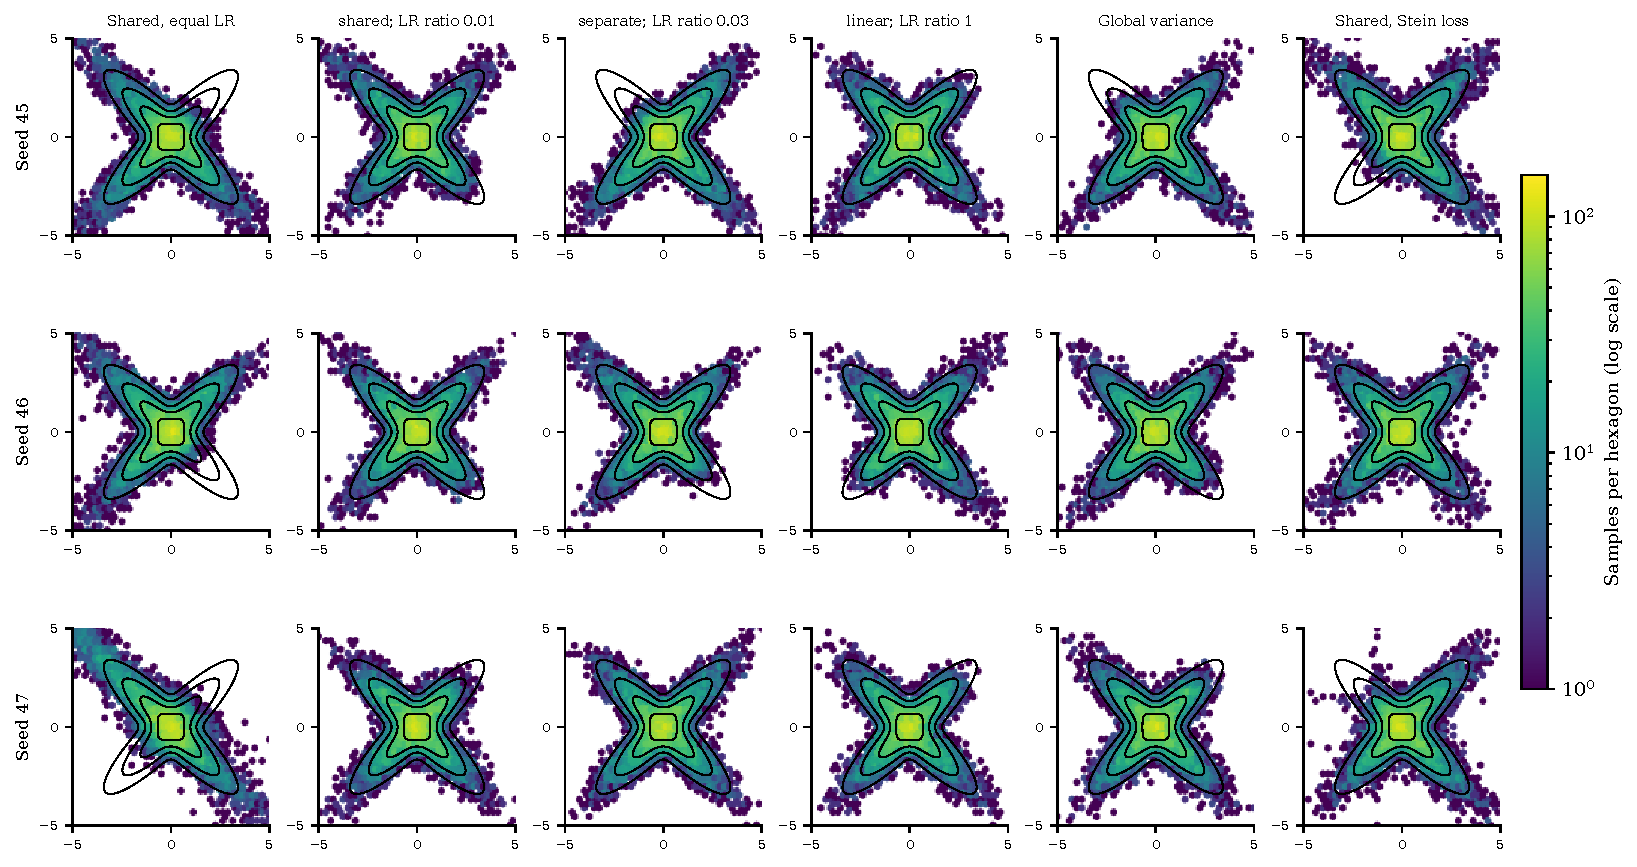
\includegraphics[width=.93\linewidth]{figures/final_samples.pdf}
\caption{Held-out seeds 45--47, selected before viewing these results. Each panel shows all 10K final samples within the common viewing window, with exact target contours in black and a common logarithmic count scale. Metrics include samples outside the window. Columns: equal-LR conditional, slow shared, selected separate, linear variance, global variance, Stein loss.}\label{fig:final_samples}
\end{figure}

\end{landscape}

\section{Reproduction, validation, and artifact inventory}
The final campaign contains 226 completed training trajectories: 66 sweep, 42 architecture, 40 held-out, 42 ablation, and 36 continuation branches. Counting shared parent updates once gives 14,900,000 optimizer updates. The 36 continuations each add 150K updates; no trajectory exceeds 200K. Experiments run on an RTX 4090 using PyTorch 2.9.0+cu126 in the server ruivi environment. Each source manifest records the commit, relevant SHA-256 hashes, complete model configuration, parameter count, and training specification.

\textbf{Final audit.} 262 endpoint/checkpoint sample arrays and diagnostics were regenerated. Loss gradients were compared against an independent kernel expression, with the Stein operator computed by spatial autograd; maximum relative difference 5.72e-07. The split-head equal-LR and legacy conditional models have bitwise identical parameters at all 18 checked seed/checkpoint pairs, and all 36 continuation branches preserve their parent model, RNG, and Adam moments at 50K. Production-runner update equality and parameter coverage are recorded separately in \texttt{validation.json}.

\textbf{Saved artifacts.} \texttt{training\_results.json} and the metric/trajectory CSVs contain every run; \texttt{selection.json} records the discovery selection; \texttt{evaluation.json} and \texttt{independent\_metrics.csv} contain all independent SW$_2$, KL refinement, and fixed-bandwidth KSD estimates and standard errors; \texttt{theory\_checks.json} and \texttt{audit.json} retain numerical checks and endpoint verification. Figures are supplied as vector PDF and PNG. Raw model/optimizer/RNG checkpoints and samples remain under \texttt{/root/ruivi/results/ksivi\_variance\_lr\_20261011}.

\textbf{Production configuration.} Use \texttt{ConditionalGaussianHeads} to enable real parameter groups. The legacy \texttt{ConditionalGaussian} retains its original combined optimizer behavior. The new shared model can be selected from the existing KSIVI config with these overrides (the first line is the model type, followed by optimizer settings):
\begin{verbatim}
vi_model_type=ConditionalGaussianHeads
train.vi.lr=0.001 train.vi.var_lr=0.00001
vi_model.variance_backbone=shared
\end{verbatim}
For the selected separate network use \texttt{variance\_backbone=separate} and \texttt{var\_lr=0.00003}. For the linear variance branch set \texttt{variance\_num\_layers=0} and \texttt{var\_lr=0.001}. Full commands, phase order, evaluation, report generation, and source changes are documented in the campaign README. Existing canonical configs are not overwritten.


\begin{thebibliography}{9}
\bibitem{ksivi} Z. Cheng, L. Yu, T. Xie, S. Zhang, and C. Zhang.
\emph{Kernel Semi-Implicit Variational Inference}. ICML, 2024.
\url{https://arxiv.org/abs/2405.18997}.
\bibitem{adam} D. P. Kingma and J. Ba.
\emph{Adam: A Method for Stochastic Optimization}. ICLR, 2015.
\url{https://arxiv.org/abs/1412.6980}.
\end{thebibliography}
\end{document}
